\chapter{Практическая часть}
\label{ch:chap2}

\section*{\textbf{Введение}}

Необходимо заполнить tx буффер своими собственными семплами, отправить их, а потом принять и посмотреть, что примит Pluto SDR. То, как заполнять буффер семплами, решает
студент.

\section*{\textbf{Формирование семплов}}

\subsection*{\textbf{Перевод строки в бинарный вид}}

Я буду формировать простой прямоугольный сигнал, который будет передавать небольшую строку. Чтобы передавать текст, нужно сначала перевести символы (char) в биты.
Для этого я написал специальную функцию:

\begin{lstlisting}
    uint8_t* stob(char* str, int* out_bits_count) {
    // get string len
    int len = strlen(str);

    // 1 char = 8 bit 
    *out_bits_count = len * sizeof(char);
    
    // massive for bits
    uint8_t* bits = (uint8_t*)malloc(*out_bits_count * sizeof(uint8_t));

    // check pointer
    if (bits == NULL){
        return NULL;
    }
        
    char c;

    // iterate on string
    for (int i = 0; i < len; i++) {
        // get char 
        c = str[i];
        // iterate on bits massive
        for (int j = 0; j < 8; j++) {
            // convert char to bits 
            bits[i * 8 + j] = (c >> (7 - j)) & 1;
        }
    }
    
    return bits;
}
\end{lstlisting}

Функция принимает саму строку и указатель на переменную, в которую запишет число битов, чтобы знать размер массива после завершения функции, и возвращает битовую последовательность.
Пример работы функции: \\

Переведем в бинарный вид строку "Hello World":

\begin{lstlisting}
    int bits_count;
    uint8_t* bits = stob("Hello World", &bits_count);
\end{lstlisting}

На выходе получим такую последовательность:

\begin{figure}[H]
    \centering
    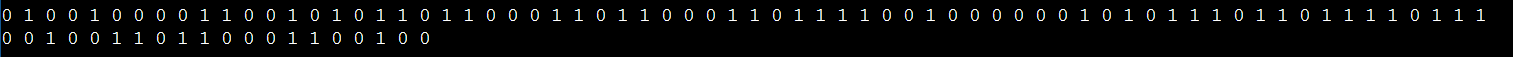
\includegraphics[width=1.0\textwidth]{bits.png}
    \caption{"Hello World" в бинарном виде}
\end{figure}

\subsection*{\textbf{Способ кодирования}}

Чтобы передать нули и единицы я буду использовать самый простой способ кодирования: 0 - ноль, 1 - максимальный I и минимальный Q.

\subsection*{\textbf{Заполнение буффера семплами}}

Для заполнения tx буффера я написал отдельную функцию, которая принимает битовую последовательнось (сообщение), длину битовой последовательности и размер семпла, а возвращает
массив семплов.

\begin{lstlisting}
int16_t* bits_to_samples(uint8_t* bits, int bits_count, int tx_mtu){

    // allocate memory
    int16_t* tx_buff = (int16_t*)malloc(sizeof(int16_t) * tx_mtu * 2);

    // iterate on bitts
    for (int i = 0; i < bits_count; i += 1)
    {   
        // fill tx_buff with samples
        for(int j = i*TAU_ON_BITS; j < i*TAU_ON_BITS + 20 && j < tx_mtu*2; j+=2){
            if(bits[i]){
                tx_buff[j] = 2047 << 4;    // I
                tx_buff[j+1] = -2047 << 4; // Q
            } else{
                tx_buff[j] = 0;      //I
                tx_buff[j+1] = 0;    //Q
            }
        }
    }

    return tx_buff;
}
\end{lstlisting}

Самое важное здесь - учитывать продолжительность импульса, т.е то кол-во семплов, которое будет приходиться на один бит информации. Я выбрал 10 семплов на бит (TAU),
а это значит, что на 1 бит информации будет приходиться 20 элементов массива (TAU\_ON\_BITS). Чем выше длительность сигнала, тем выше шанс шанс верно декодировать его
на применой стороне, но при этом падает скорость передачи данных. Работать заполнение будет так: берем первые 20 элементов массива и заполняем его идентичными значениями
(в соответсвии со состоянием бита), потом берем следующие 20 и т.д.


\begin{figure}[H]
    \centering
    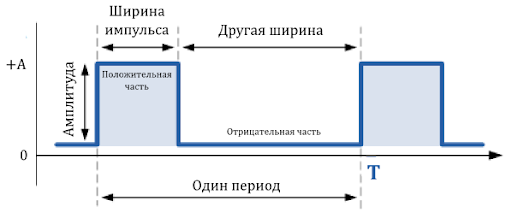
\includegraphics[width=1.0\textwidth]{rect_sig.png}
    \caption{Пример прямоугольного сигнала с обозначениями}
\end{figure}

\subsection*{\textbf{Визуализация полученного сигнала с помощью скрипта на Python}}

\begin{figure}[H]
    \centering
    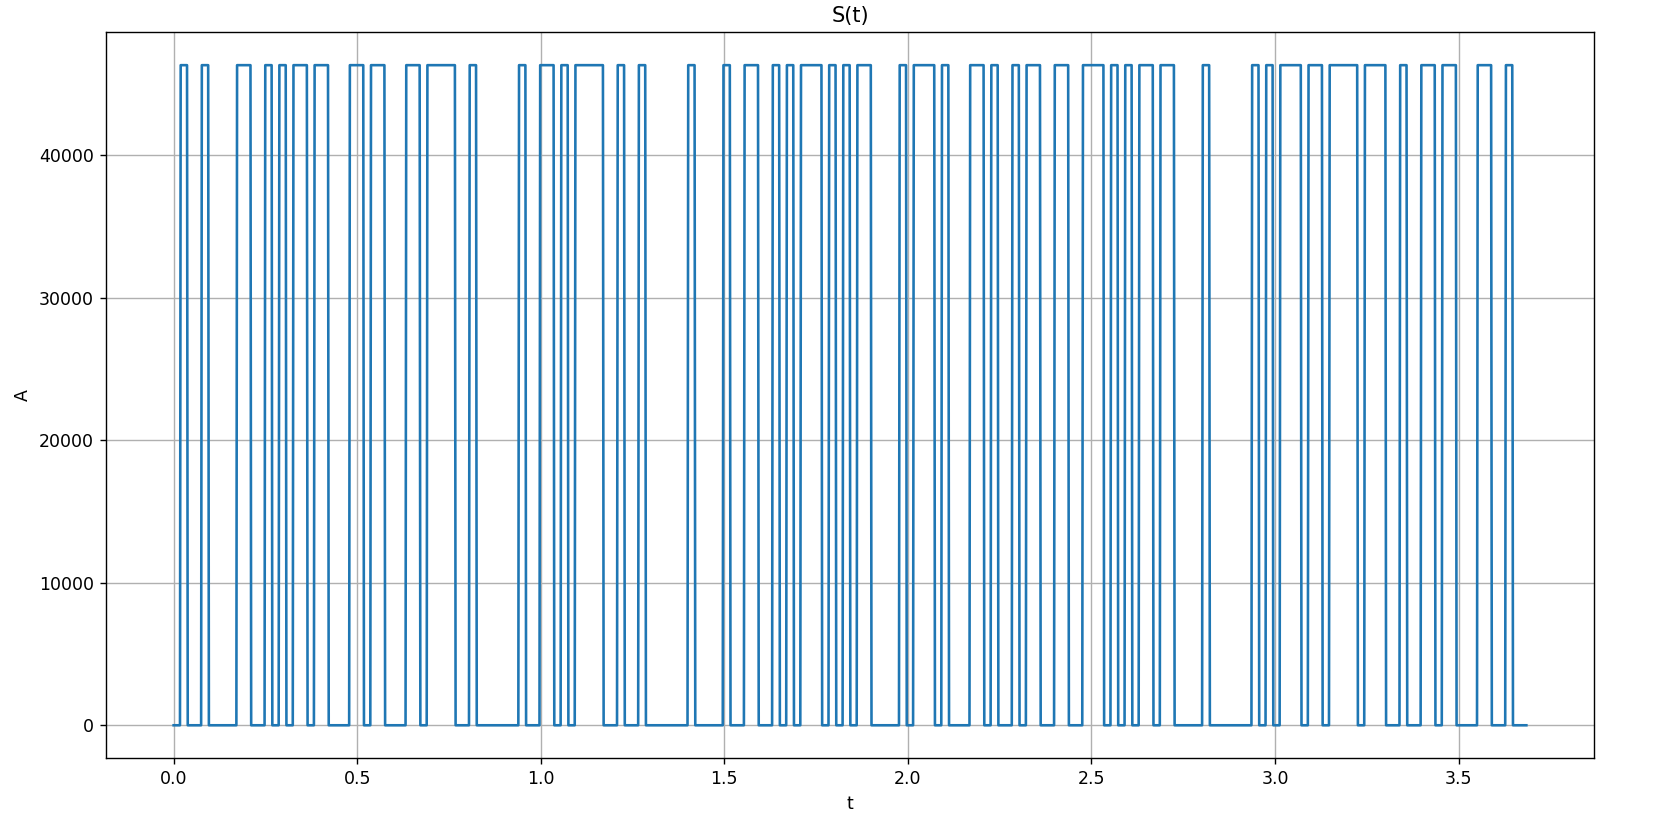
\includegraphics[width=1.0\textwidth]{signal.png}
    \caption{Пример полученного прямоугольного сигнала}
\end{figure}

Этот прямоугольный сигнал содержит наше сообщение.

\subsection*{\textbf{Требование к длине сообщения}}

Для Pluto SDR рекомендуется использовать для отправки/приема 1920 семплов или число семплов кратное 1920. Если на 1 бит приходится 10 семплов, то сообщение должно
быть длиной 192 бита, а т.к я пытаюсь передать символы размером 8 бит, то необходима строка длиной 24 символа.


\section*{\textbf{Прием семплов}}

На приеме получили следующий сигнал:

\begin{figure}[H]
    \centering
    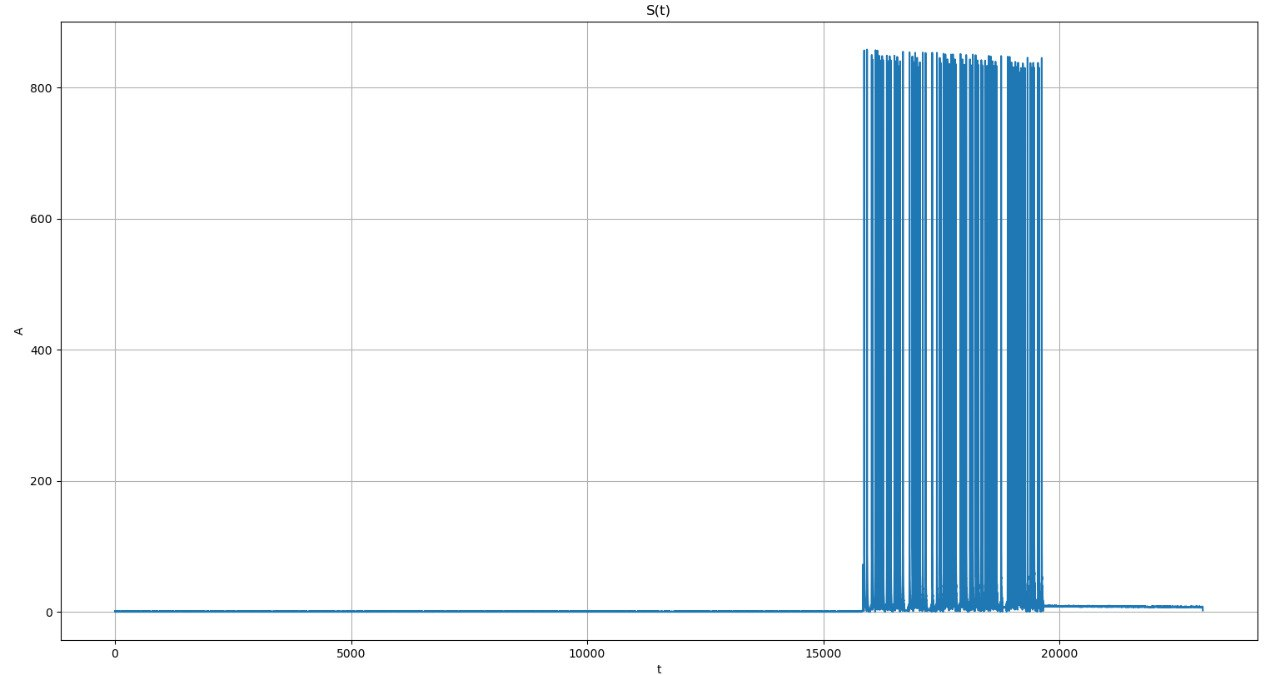
\includegraphics[width=1.0\textwidth]{rx_samples.png}
    \caption{Сигнал на приеме}
\end{figure}

Где то среди этого сигнала наше сообщение, но чтобы правильно его декодировать необходимо синхронизировать устройтсва с помощью специальных последовательностей. Эта тема
будет рассматриваться в дальнейшем.

\endinput
